\begin{figure}[H]
    \centering
    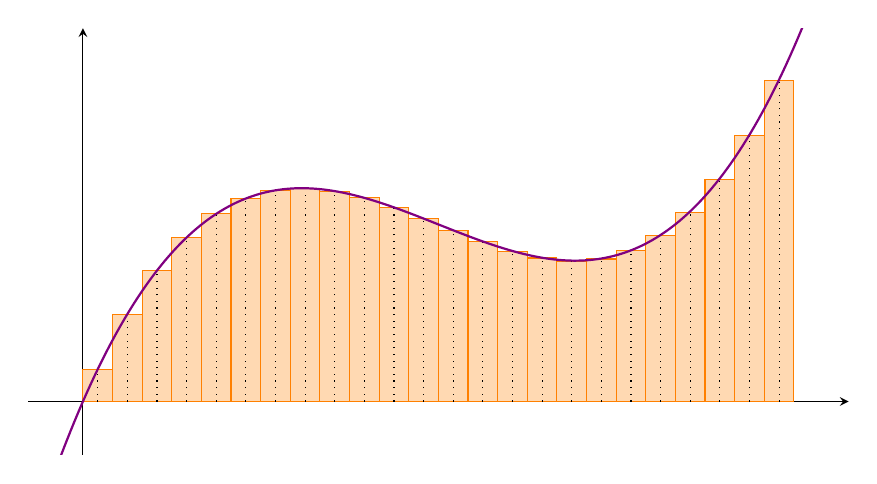
\begin{tikzpicture}[scale=1]
        \begin{axis}[
            axis lines=middle,
            xtick=\empty,
            ytick=\empty,
            xmin=-1, xmax=14,
            ymin=-1, ymax=7,
            width=12cm, height=7cm
        ]
        
        % Số cột
        \pgfmathsetmacro{\N}{24}
        % Bước chia
        \pgfmathsetmacro{\dx}{13/\N}
        
        % Vẽ các cột Riemann (lấy theo trung điểm)
        \foreach \i in {0,...,23} {
            \pgfmathsetmacro{\xmid}{(\i+0.5)*\dx} % trung điểm
            \pgfmathsetmacro{\y}{1/46*\xmid^3 - 39/92*\xmid^2 + 54/23*\xmid}
            % Hình chữ nhật (cột)
            \addplot[ybar, bar width=\dx, fill=orange!30, draw=orange] coordinates {(\xmid, \y)};
            % Đường chấm dọc
            \addplot[dotted, black] coordinates {(\xmid,0) (\xmid,\y)};
        }

        % Vẽ đường cong màu tím
        \addplot[domain=-0.8:13.5, samples=200, color=violet, thick] {1/46*x^3 - 39/92*x^2 + 54/23*x};
        
        \end{axis}
    \end{tikzpicture}
    \caption{Tổng Riemann (lấy theo trung điểm).}
    \label{fig:riemann_sum}
\end{figure}
